\documentclass[10pt, letterpaper]{report}
% !TeX program = xelatex
%==================PREAMBOLO=======================%
\usepackage[utf8]{inputenc}
\usepackage{psvectorian}
\usepackage{pgfplots}
\usepackage[Rejne]{fncychap}
\usepackage[export]{adjustbox}
\usepackage[T1]{fontenc}
\usepackage{lmodern}
\usepackage{blindtext}
\usepackage{pdfpages}
\usepackage[shortlabels]{enumitem}
\usepackage{moresize}
\usepackage{graphicx} % Required for inserting images
\usepackage{hyperref}
\usepackage{listings}
\usepackage[table,xcdraw]{xcolor}
\usepackage{amssymb}
\usepackage{amsmath}
\usepackage[italian]{babel}
\usepackage{nicefrac, xfrac}
\usepackage{tikz}
\usepackage{tikz-3dplot}
\usepackage{mathrsfs} 
\usepackage{titletoc}
\usepackage{fancyhdr}
\usepackage{psvectorian,lipsum}
\usepackage{fourier-orns}
\usepackage{lipsum}
\usepackage{multicol}
\usepackage[paper=a4paper,left=25mm,right=25mm,bottom=25mm,top=25mm]{geometry}
\definecolor{light-gray}{gray}{0.95}
\definecolor{cop}{HTML}{f7ecd7}
\definecolor{copAut}{HTML}{ababab}
\definecolor{copAut2}{HTML}{c3c3e6}
\definecolor{purcop}{HTML}{d0d3db}
\definecolor{sapienza}{HTML}{660f1d}
\definecolor{lightSapienza}{HTML}{e3d3d5}
\definecolor{darkgreen}{HTML}{008000}
\definecolor{cartaRiciclata}{HTML}{fcfcf7}
\newcommand{\redText}[1]{\color{red}#1\color{black}}
\newcommand{\code}[1]{\colorbox{light-gray}{\texttt{#1}}}
\newcommand{\codee}[1]{\colorbox{white}{\texttt{#1}}}
\newcommand{\K}{{\mathbb K}}
\newcommand{\notimplies}{%
  \mathrel{{\ooalign{\hidewidth$\not\phantom{=}$\hidewidth\cr$\implies$}}}}
\newcommand{\flowerLine}{ \begin{center}\decofourleft\hphantom{ }\decoone\hphantom{ }\decofourright\hphantom{}\hphantom{aa}
\decofourleft\hphantom{ }\decoone\hphantom{ }\decofourright\hphantom{}\hphantom{aa}
\decofourleft\hphantom{ }\decoone\hphantom{ }\decofourright\hphantom{}\hphantom{aa}
\decofourleft\hphantom{ }\decoone\hphantom{ }\decofourright\hphantom{}\hphantom{aa} 
\decofourleft\hphantom{ }\decoone\hphantom{ }\decofourright\hphantom{}\hphantom{aa}
\decofourleft\hphantom{ }\decoone\hphantom{ }\decofourright\hphantom{}\hphantom{aa}
\decofourleft\hphantom{ }\decoone\hphantom{ }\decofourright\hphantom{}\hphantom{aa}
\decofourleft\hphantom{ }\decoone\hphantom{ }\decofourright\hphantom{}\hphantom{aa}
\decofourleft\hphantom{ }\decoone\hphantom{ }\decofourright\hphantom{}\hphantom{aa}
\end{center}}
\definecolor{g}{RGB}{60, 50, 50}
\newcommand{\textg}[1]{\color{g}{\textbf{#1}}\color{black}}
\newcommand{\teo}[1]{{\large\color{sapienza}\textbf{Teorema #1 :\hphantom{a}}}}
\newcommand{\defi}[1]{{\large\color{sapienza}\textbf{Definizione #1 :\hphantom{a}}}}
\newcommand{\claim}[1]{{\color{sapienza}\textbf{Claim #1 :\hphantom{a}}}}
\newcommand{\lemma}[1]{{\color{sapienza}\textbf{Lemma #1 :\hphantom{a}}}}
\newcommand{\dimo}[1]{{\color{sapienza}\textbf{Dimostrazione #1 :\hphantom{a}}}}
\newcommand{\prop}[1]{{\color{sapienza}\textbf{Proposizione #1 :\hphantom{a}}}}
\newcommand\greybox[1]{%
  \vskip\baselineskip%
  \par\noindent\colorbox{light-gray}{%
    \begin{minipage}{\textwidth}#1\end{minipage}%
  }%
  \vskip\baselineskip%
}
\newcommand\sapbox[1]{%
  \vskip\baselineskip%
  \par\noindent\colorbox{lightSapienza}{%
    \begin{minipage}{\textwidth}#1\end{minipage}%
  }%
  \vskip\baselineskip%
}
\newcommand{\ridFunc}{{f:\Sigma^*\rightarrow \Sigma^*}}
\newcommand{\rid}{{\le_m^P}}
\newcommand{\Z}{{\mathbb Z}}
\newcommand{\blank}{{\sqcup}}
\newcommand{\R}{{\mathbb R}}
\newcommand{\N}{{\mathbb N}}
\newcommand{\C}{{\mathbb C}}
\newcommand{\Sn}{{\mathcal S_n}}
\newcommand{\An}{{\mathcal A_n}}
\newcommand{\E}{{\mathcal E}}
\newcommand{\B}{{\mathcal B}}
\newcommand{\mcm}{{\text{mcm}}}
\newcommand{\rg}{{\text{rg}}}
\newcommand{\ve}{{\bar v}}
\newcommand{\spaz}{{\text{\hphantom{aa}}}}
\newcommand{\MCD}{{\text{MCD}}}
\newcommand{\tc}{{\text{ tale che }}}
\newcommand{\supp}{{\text{Supp}}}
\newcommand{\acc}{\\\hphantom{}\\}
\newcommand{\esempio}[1]{{\acc\large\color{sapienza}\textbf{Esempio #1 \hphantom{a}}\acc}}
\newcommand{\bra}[1]{\langle #1 \rangle}
\newcommand{\aut}{{\text{Aut}}}
\newcommand{\Span}{{\text{Span}}}
\newcommand{\End}{{\text{End}}}
\newcommand{\cen}{{\text{Centro}}}
\newcommand{\norm}{{\unlhd}}
\newcommand{\ciclS}{{\left \langle }}
\newcommand{\ciclE}{{\right \rangle }}
\newcommand{\boxedMath}[1]{\begin{tabular}{|c|}\hline \texttt{#1} \\ \hline\end{tabular} :} 
\newcommand{\shell}[1]{\colorbox{black}{\textcolor{white}{\texttt{#1}}}}
\newcommand{\eqImportante}[1]{\begin{center}\huge\lefthand\hphantom{a}
    \normalsize\texttt{#1}
    \hphantom{aaa}\huge\righthand\end{center}}

\fancyhf{}
\pagestyle{fancy}
\usepackage{pgf-pie}  
\usetikzlibrary{positioning}

\renewcommand{\headrule}{%
\vspace{-8pt}\hrulefill
\raisebox{-2.1pt}{\quad\decothreeleft\decotwo\decothreeright\quad}\hrulefill}

%sta roba serve per il codice C
\definecolor{mGreen}{rgb}{0,0.6,0}
\definecolor{mGray}{rgb}{0.5,0.5,0.5}
\definecolor{mPurple}{rgb}{0.58,0,0.82}
\definecolor{backgroundColour}{rgb}{0.95,0.95,0.92}

\lstdefinestyle{CStyle}{
    backgroundcolor=\color{backgroundColour},   
    commentstyle=\color{mGreen},
    keywordstyle=\color{magenta},
    numberstyle=\tiny\color{mGray},
    stringstyle=\color{mPurple},
    basicstyle=\footnotesize,
    breakatwhitespace=false,         
    breaklines=true,                 
    captionpos=b,                    
    keepspaces=true,                 
    numbers=left,                    
    numbersep=5pt,                  
    showspaces=false,                
    showstringspaces=false,
    showtabs=false,                  
    tabsize=2,
    language=C
}
\lstdefinestyle{CppStyle}{
    backgroundcolor=\color{backgroundColour},   
    commentstyle=\color{mGreen}\ttfamily,
    morecomment=[l][\color{magenta}]{\#}
    keywordstyle=\color{blue}\ttfamily,
    numberstyle=\tiny\color{mGray},
    stringstyle=\color{red}\ttfamily,
    basicstyle=\ttfamily,
    breakatwhitespace=false,         
    breaklines=true,                 
    captionpos=b,                    
    keepspaces=true,                 
    numbers=left,                    
    numbersep=5pt,                  
    showspaces=false,                
    showstringspaces=false,
    showtabs=false,                  
    tabsize=2,
    language=C
}
\lstset{language=C++,
                basicstyle=\ttfamily,
                keywordstyle=\color{blue}\ttfamily,
                stringstyle=\color{red}\ttfamily,
                commentstyle=\color{green}\ttfamily,
                morecomment=[l][\color{magenta}]{\#}
}
%fine roba che serve per il codice C
\usepackage{minted}
\usetikzlibrary{petri}
 %TOGLI COMMENTO SE USI XELATEX
%\usepackage{fontspec}
\title{\jobname} %========TITOLO========%
\author{Marco Casu}
\date{\vspace{-5ex}}
\begin{document}

%==================COPERTINA=======================%
\begin{titlepage}
    \pagecolor{copAut}
\begin{center}
    %TOGLI COMMENTO SE USI XELATEX
   %\setmainfont{Palace Script MT}
   \HUGE Marco Casu\acc
    %\setmainfont{Grand Casino}
     %TOGLI COMMENTO SE USI XELATEX
    %\setmainfont{h Halfroad}
    \HUGE \decothreeleft\hphantom{ }{\fontsize{48}{50}\selectfont \jobname}\hphantom{ }\decothreeright
     %TOGLI COMMENTO SE USI XELATEX
   % \setmainfont{Times New Roman}
\end{center}
\thispagestyle{empty}
\begin{figure}[h]
    \centering{
        %l'immagine deve avere una risoluzione 2048x2048
        \includegraphics[width=1\textwidth ]{images/Copertina.jpeg}
    }
\end{figure}
\vfill 
\centering \includegraphics[width=0.4\textwidth ]{../../../preamble/Stemma_sapienza.png} \acc
\centering \Large \color{sapienza}Facoltà di Ingegneria dell'Informazione,
Informatica e Statistica\\
Dipartimento di Informatica
\end{titlepage}

%===================FINE COPERTINA======================%
\newpage
\pagecolor{cartaRiciclata}%\setmainfont{Algerian}
\Large
Questo documento è distribuito sotto la licenza 
\color{blue}\href{https://www.gnu.org/licenses/fdl-1.3.txt}{GNU}\color{black},  
è un resoconto degli appunti (eventualmente integrati con libri di testo) tratti dalle lezioni del corso di \jobname
\hphantom{a}per la laurea 
triennale in Informatica. Se dovessi notare errori, ti prego di segnalarmeli.\acc 
Nota bene : Essendo questi appunti di un corso esterno alla facoltà di Informatica, 
è presente un capitolo "Complementi" che può risultare utile al lettore.
\vfill
\begin{figure}[h!]
    \raggedright
    \includegraphics[width=0.4\textwidth,right ]{../../../preamble/tomodachi.pdf} 
\end{figure}
\newpage %\setmainfont{Times New Roman}
\normalsize
\tableofcontents 
\newpage

%==================FOOTER e HEADER=======================%
\fancyhf{}
\fancyhead[L]{\nouppercase{\leftmark}}
\fancyhead[R]{Sezione \thesection}
\fancyfoot[C]{\thepage}
\fancyfoot[L]{Appunti di \jobname}
\fancyfoot[R]{ Marco Casu}
%\fancyfoot[R]{\setmainfont{Palace Script MT}\huge Marco Casu \setmainfont{Times New Roman}}
%==================FOOTER e HEADER=======================%

%Ricorda del comando \flowerLine per separare le sottosezioni. Le sezioni si separano nelle diverse pagine

%==================INIZIO======================%
\chapter{Introduzione}
Con il termine \textit{Automazione}, si intende la trasformazione 
di un processo pre-esistente, al fine di renderlo autonomo, riducendo o 
sostituendo del tutto l'intervento umano, verrà trattata l'automazione 
dei processi industriali e manifatturieri, e del loro controllo e 
supervisione. I sistemi presi in considerazione evolvono nel 
tempo e reagiscono ad eventi, che ne cambiano lo stato, e scaturiscono 
dei feedback, per un eventuale correzione dell'errore.\acc 
Con sistema \textit{autonomo} si intende un sistema in cui viene 
ridotto l'intervento umano. L'\textit{Automatica} si occupa di 
sfruttare gli strumenti dell'informatica per l'automazione, acquisendo informazioni 
dal mondo fisico tramite appositi sensori, per poi essere elaborate 
su un sistema di controllo (calcolatore), o una rete di calcolatori, 
che implementa dei protocolli standard per l'industria. Differentemente da 
altri contesti, come la trasmissione (ad esempio, di un video in streaming) nelle 
reti dell'automazione i ritardi risultano critici, e vanno ridotti al 
minimo.
\begin{center}
    \begin{figure}[h!]
        \centering
        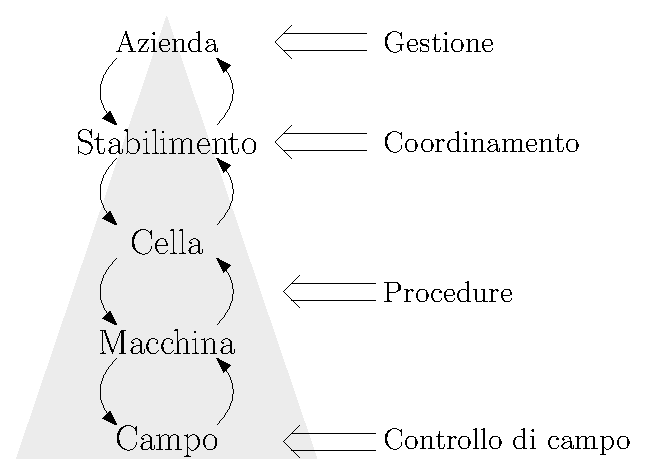
\includegraphics[width=0.4\textwidth ]{images/CIM.eps}
        \caption{Piramide CIM}
        \label{fig:cim}
   \end{figure}
   \end{center}
La \textit{piramide CIM}, mostrata in figura \ref{fig:cim}
schematizza la gestione di un processo industriale e delle sue procedure, 
ogni strato comunica con quelli adiacenti scambiandosi informazioni, nei 
livelli più alti, le informazioni sono più \textit{raffinate} ed 
astratte, nei livelli più bassi sono più grezze, ad esempio\begin{itemize}
    \item Al livello azienda viene decisa la produzione di un articolo (che 
    coinvolgerà l'utilizzo di un braccio robotico)
    \item Al livello macchina, l'informazione che arriverà al braccio 
    sarà semplicemente relativi ai gradi in cui i suoi giunti devono 
    ruotare
    \item Al livello di campo, l'informazione comprenderà semplicemente 
    il voltaggio da applicare alla macchina in questione per avere l'effetto 
    desiderato.
\end{itemize}
Con \textbf{cella}, si intende un unità composta da più macchine, in 
cui viene scambiato e lavorato del materiale per compiere delle azioni,
il \textit{controllo delle procedure} si occupa delle \textbf{macchine}, ed uno 
\textbf{stabilimento} è un complesso di celle/parti e catene 
di montaggio. nel livello di campo, vengono utilizzati vari dispositivi, 
quali\begin{itemize}
    \item motori elettrici, servomotori, encoder 
    \item azionatori di valvole, dynamo tachimetrici, sensori di temperatura
\end{itemize}
Tali sensori presenteranno stesso un comportamento lineare, ad esempio, 
se una tensione $x$ causa una rotazione di $y$ giri per minuti, allora 
una tensione $2x$ causerà una  rotazione di $2y$. Anche se tali dispositivi 
non si prestano ad un comportamento lineare, ne verrà causata una volontaria 
linearizzazione, correggendone il comportamento.\acc 
Argomento centrale saranno i regolatori \textit{PID}, la cui definizione, 
come molte altre trattate in questo capitolo, sarà ripresa ed 
approfondita in seguito. tali regolatori agiscono su delle grandezze 
di campo.\begin{center}
    \begin{figure}[h!]
        \centering
        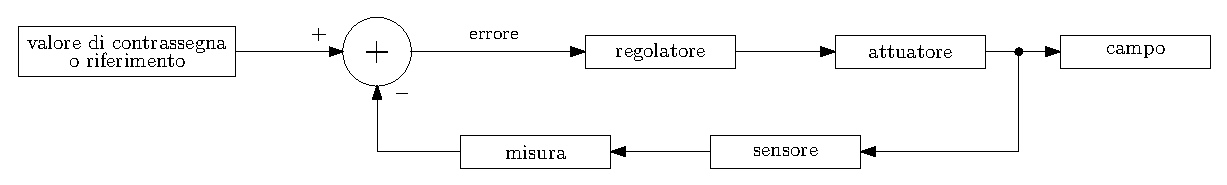
\includegraphics[width=1\textwidth ]{images/schemaPID.eps}
        \caption{schematizzazione del regolatore PID}
        \label{fig:schemaPID}
   \end{figure}
\end{center}
Si consideri il seguente esempio di regolatore, vi è una stufa che deve 
riscaldare una stanza, ed un sensore che ne misura la temperatura, il valore 
da raggiungere, detto \textit{setpoint}, è di 20 gradi celcius. Si supponga che il 
sensore, una volta rilevata la temperatura, debba accendere e spengere la stufa 
in modo che si raggiunga la temperatura adeguata.
\begin{center}
    \begin{figure}[h!]
        \centering
        \includegraphics[width=0.6\textwidth ]{images/stufaEsempio.eps}
        \caption{Azioni sulla stufa}
        \label{fig:stufa}
   \end{figure} 
\end{center}
In figura \ref{fig:stufa}, il differenziale rappresenta un margine 
di differenza rispetto il setpoint, quando la temperatura è 
sotto il limite inferiore, la stufa viene accesa, quando è oltre il limite 
superiore, viene spenta (è chiaro che la velocità con la quale la temperatura 
cambia dipende dalle capacità della stufa e dalla dispersione del calore nella stanza).\acc 
Ridurre il valore del differenziale costringerebbe la temperatura ad assestarsi 
sempre di più sul valore desiderato, ma ciò, comporterebbe un'accensione/spengimento della 
stufa più frequente, aumentando lo \textit{sforzo di controllo}, è quindi, in questo 
caso, accettabile un differenziale di $2^\circ$.\acc 
Tale modello di controllo è il più semplice che ci sia, esistono ovviamente altri modi di regolare un 
segnale in modo che esso raggiunga il valore desiderato, ad esempio, calcolare l'errore $e$ (ossia la differenza 
fra il valore desiderato ed il valore effettivo) e scalarlo ad una certa costante $K_p$ per poi utilizzare tale 
valore nella regolazione del segnale.
\begin{center}
    \begin{figure}[h!]
        \centering
        \includegraphics[width=0.6\textwidth ]{images/stufaEsempioPROP.eps}
        \caption{Regolatore proporzionale}
        \label{fig:regPropStuda}
   \end{figure} 
\end{center}
Anche se la variazione della temperatura è continua nel tempo, il suo 
superare una certa soglia è un evento, i PLC (controllori logici programmabili) 
agiscono sulle misure di campo, un noto linguaggio utilizzato per descriverne 
il funzionamento è noto come \textit{Sequential Flow Chart (SFL)}.\acc 
Nei sistemi di automazione industriale vengono prediletti controllori e sensori distribuiti piuttosto 
che centralizzati, se ne vuole dare una dimostrazione pratica con il segunete 
esempio : Si considerino i due seguenti modi per trasportare un oggetto 
su un nastro trasportatore :\begin{center}
    \begin{figure}[h!]
        \centering
        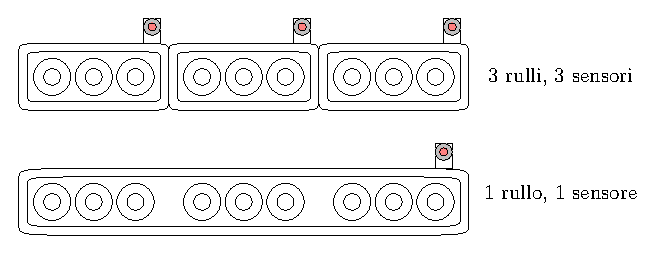
\includegraphics[width=0.6\textwidth ]{images/rulli.eps}
        \caption{Rulli}
        \label{fig:rulli}
   \end{figure} 
\end{center}
Ogni nastro ha un sensore, se un oggetto è rilevato sopra il nastro, allora il motore si attiva. Risulta più efficente 
la soluzione con 3 nastri in quanti sarà adoperata solamente la zona del nastro in cui è rilevato l'oggetto, piuttosto 
che l'intero nastro.\acc 
Per la modellizzazione di sistemi autonomi verranno adoperati automi a stati finiti, ampiamente trattati nel 
corso di 
\color{blue}\href{https://github.com/CasuFrost/University_notes/blob/main/Terzo%20Anno/Automi%2C%20Calcolabilit%C3%A0%20e%20Complessit%C3%A0/Automi%2C%20Calcolabilit%C3%A0%20e%20Complessit%C3%A0.pdf}{Automi, Calcolabilità e Complessità}
\color{black}, e \textit{Reti di Petri}. Una rete di Petri, non è altro che un grafo bipartito, in cui ogni nodo 
appartiene ad un'insieme fra \begin{itemize}
    \item nodi \textit{posto}
    \item nodi \textit{transizione}
\end{itemize}
Inoltre, i nodi posto possono essere annotati con dei pallini neri, detti \textit{token}, essi rappresentano 
lo stato del sistema in quanto indicano che delle risorse (in senso generale) sono disponibili in un posto, 
permettendo eventualmente una transizione. Ogni arco del grafo collega un nodo posto ad un nodo transizione.
\begin{figure}[h!]
    \centering
    \begin{tikzpicture}
        \node[place,tokens=2,label=above:$p_1$]        (p1) {};
        \node[place,label=above:$p_2$,right=of p1] (p2) {};
        \node[place,tokens=1,label=above:$p_3$,right=of p2] (p3) {};
        \node[place,label=above:$p_4$,below=of p3,right=of p3] (p4) {};
        \node[place,tokens=1,label=above:$p_5$,below=of p1] (p5) {};
       
      
        \node[transition,below right=of p1,label=below:$t_1$] {}
          edge[pre]                 (p1)
          edge[post] node[auto] {} (p2)
          edge[post] node[auto] {} (p5);
        \node[transition,below right=of p2,label=below:$t_2$] {}
          edge[pre]                 (p2)
          edge[post] node[auto] {} (p3)
          edge[post] node[auto] {} (p4);
      \end{tikzpicture}
      \caption{Esempio di una rete di Petri}
\end{figure}
















\chapter{Complementi}
\section{La Trasformata di Laplace} 
La trasformata di Laplace è una \textit{trasformata integrale}, nello specifico, è una 
funzione che associa ad una funzione di variabile reale, una funzione di variabile 
complessa.\acc 
\defi{(Trasformata di Laplace)} : Sia $f$ una funzione di variabile reale, nulla 
in $(-\infty,0)$, si chiama trasformata di Laplace di $f$ la funzione 
$$ \mathcal{L}[f](p)=\int_0^{+\infty} e^{-px}f(x)\ dx \ \ \ \ p\in \C$$
Essendo $p = \alpha + i\beta$ una variabile complessa, la funzione integranda si può riscrivere 
$$\int_0^{+\infty} e^{-px}f(x)\ dx = 
\int_0^{+\infty} e^{-(\alpha + i\beta)x}f(x)\ dx$$
Ricordando l'identità di Eulero $$ e^{ix}=\cos(x)+i\sin(x)$$
Si ha 
\begin{eqnarray}
    e^{-(\alpha + \beta i)x} = e^{-\alpha x}\cdot e^{-\beta i x} =\\ 
    e^{-\alpha x}\cdot \Big(
    \cos(-\beta x)+ i \sin(-\beta x)    
    \Big) = e^{-\alpha x}\cdot \Big(
        \cos(\beta x)- i \sin(\beta x)    
        \Big) = \\ 
        e^{-\alpha x}\cos(\beta x)- i e^{-\alpha x}\sin(\beta x)
\end{eqnarray}
Quindi $$ \mathcal{L}[f](p)=\mathcal{L}[f](\alpha + i\beta)=
\int_0^{+\infty} e^{-(\alpha + i\beta)x}f(x)\ dx=
$$
$$
\int_0^{+\infty} e^{-\alpha x}\cos(\beta x)f(x)-ie^{-\alpha x}\sin(\beta x)f(x)\ dx =$$
$$ 
\int_0^{+\infty} e^{-\alpha x}\cos(\beta x)f(x)\ dx-i\int_0^{+\infty}e^{-\alpha x}\sin(\beta x)f(x)\ dx
$$
Se l'integrale $\mathcal{L}[f](\alpha + i\beta)$ converge per un certo
 $\alpha \in \R$, allora converge per $p = \alpha + i\beta$ per ogni altro $\beta \in \R$. Se per 
 $f$ esiste almeno un $p\in\C$ tale che $\mathcal{L}[f](p)<\infty$, allora $f$ si dice 
 \textit{trasformabile secondo Laplace}.\acc
 In generale, se $\mathcal{L}[f](p)<\infty$ per $p=p_0$, allora è definita anche nel semipiano 
 complesso $$\{p\in \C \ |\ \Re(p)>\Re(p_0)\}$$
 Sia $\alpha_0$ l'estremo inferiore dell'insieme $\{\alpha \in \R \ |\ \mathcal{L}[f](p)<\infty\land \Re(p)>\alpha\}$, allora 
 il semipiano $\{p\in \C \|\ \Re(p)>\alpha_0\}$ è detto \textbf{semipiano di convergenza}.
 \begin{center}
    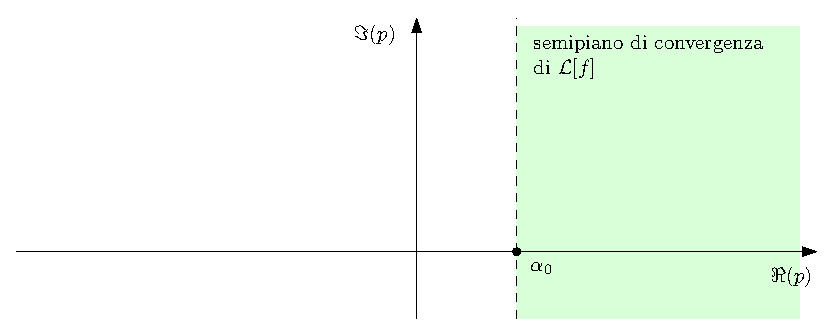
\includegraphics[width=0.6\textwidth ]{images/semiPianoConv.eps}
 \end{center}
 Vediamo un esempio di trasformata, si consideri $$ 
 H(x)=\begin{cases}
    1 \text{ se }x\ge 0\\ 0 \text{ altrimenti }
 \end{cases}
 $$
 \begin{center}
 \begin{figure}[h!]
    \centering
    \begin{tikzpicture}[scale=0.7, transform shape]
        \begin{axis}[
        ymin=-3,
        ymax = 3,
        xmin=-3,
        xmax = 3,
        axis lines = center,
        xtick distance=1, ytick distance=1,
        grid style=dashed,
        ymajorgrids=true,
        xmajorgrids=true,
        xlabel = \(\),
        ylabel = {\(\)},
        ]
        %Below the red parabola is defined
        \addplot [
        domain=0:3,
        samples=20,
        color=blue,
        ]
        {1};
        \end{axis}
        \end{tikzpicture}
        \caption{Funzione di Heaviside}
\end{figure}
\end{center}
Si calcola 
$$ \mathcal{L}[H](p)=\int_0^{+\infty}e^{-px}\cdot 1 \ dx = 
\lim_{T\rightarrow+\infty}\mathcal{L}[H](p)=\int_0^{T}e^{-px}\cdot 1 \ dx = 
\lim_{T\rightarrow+\infty}\begin{bmatrix}
    -\dfrac{e^{-px}}{p}
\end{bmatrix}_0^T=$$
$$\lim_{T\rightarrow+\infty} -\dfrac{e^{-pT}}{p} - \Big[-\dfrac{e^{-p0}}{p}\Big] =  
\lim_{T\rightarrow+\infty} -\dfrac{e^{-pT}}{p} +\dfrac{1}{p}=\frac{1}{p}$$
Il cui semipiano di convergenza risulta essere $\Re(p)>0$.
\subsection{Proprietà della Trasformata}
\subsubsection{Linearità}
La trasformazione di Laplace gode della proprietà di \textit{linearità}, siano $f(p)$ e $g(p)$ due funzioni 
trasformabili, siano $\lambda,\mu \in \C$ due costanti complesse, se la funzione 
$\lambda \cdot f(p)+\mu \cdot g(p)$ è trasformabile, allora 
$$ 
\mathcal{L}[\lambda \cdot f+\mu \cdot g](p)=\lambda\mathcal{L}[f](p)+\mu\mathcal{L}[g](p)
$$
Il semipiano di convergenza sarà uguale all'intersezione dei due semipiani di convergenza delle funzioni 
di partenza, più precisamente se \begin{itemize}
    \item $f$ ha come semipiano di convergenza $\Re(p)>\alpha$
    \item $g$ ha come semipiano di convergenza $\Re(p)>\beta$
    \item allora $\lambda \cdot f+\mu \cdot g$ ha come semipiano di convergenza $\Re(p)>\max\{\beta,\alpha\}$
\end{itemize}
\subsubsection{Ritardo}
Sia $f$ una funzione trasformabile, si consideri una costante reale $a>0$, la funzione $g(x)=f(x-a)$ è detta 
funzione \textit{ritardata}.\begin{center}
\begin{figure}[h!]\centering
    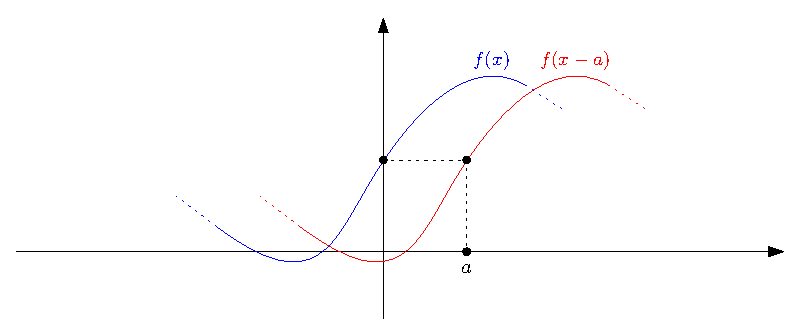
\includegraphics[width=0.6\textwidth ]{images/funRit.eps}
    \caption{funzione ritardata}
 \end{figure}\end{center}
Per il calcolo della trasformata di $g(x)=f(x-a)$ si considera il cambio di variabile $$\begin{matrix}
    t=x-a\\ x=t+a
\end{matrix} $$
Si ricordi come, se $f$ è nulla in $(-\infty,0)$, allora $g$ sarà nulla in $(0,a)$.
$$ 
\mathcal{L}[g](p)=\int_0^{+\infty}e^{-px}g(x)\ dx =\int_a^{+\infty}e^{-px}f(x-a)\ dx  =
\int_a^{+\infty}e^{-p(t+a)}f(t)\ dx = 
$$ 
$$ 
\int_a^{+\infty}e^{-pt-pa}f(t)\ dx 
= \int_a^{+\infty}e^{-pt}e^{-pa}f(t)\ dx = e^{-pa}\int_a^{+\infty}e^{-pt}f(t)\ dx = 
e^{-pa}\mathcal{L}[f](p)$$
Dunque si ricavano le cosiddette \textit{formule del ritardo} : 
$$ 
\mathcal{L}[f(x-a)](p)=e^{-pa}\mathcal{L}[f(x)](p)
$$ $$ 
\mathcal{L}[e^{ax}f(x)](p)=\mathcal{L}[f](p-a)
$$
\subsubsection{Trasformazione di una derivata e di una primitiva}
La seguente proprietà risulta cruciale nell'utilizzo della trasformata di Laplace per la risoluzione di 
equazioni differenziali. Le dimostrazioni dei seguenti risultati non saranno trattate in quanto non 
sono argomento di questo corso.\acc 
Sia $f$ una funzione derivabile, la cui derivata è continua in $[0,\infty)$. Sia inoltre $f'$ trasformabile, con 
semipiano di convergenza $\Re(p)>\alpha$, allora anche $f$ è trasformabile, ha semipiano di 
convergenza $\Re(p)>\max\{\alpha,0\}$, e vale la seguente identità :
\eqImportante{$
\mathcal{L}[f'](p)=p\mathcal{L}[f](p)-f(0)
$}
Si generalizza per derivate di ordine maggiore 
$$ 
\mathcal{L}[f''](p)=p^2\mathcal{L}[f](p)-pf(0)-f'(0)
$$
Analogamente, sia $F(x)=\int_0^x f(t)\ dt$, se $f$ è trasformabile ed ha semipiano di convergenza  $\Re(p)>\alpha$, 
allora anche $F$ lo è, ha semipiano di convergenza $\Re(p)>\max\{\alpha,0\}$ e vale che 
\eqImportante{$
\mathcal{L}[F](p)=\dfrac{1}{p}\mathcal{L}[f](p)
$}
\subsubsection{Convoluzione}
Siano $f$ e $g$ due funzioni integrabili secondo Riemann e nulle in $(-\infty,0)$, l'operatore $*$ detto \textbf{convoluzione} è 
definito nel modo seguente 
$$ (f*g)(x)=\int_0^{+\infty}f(x-t)g(t)\ dt=\int_0^{+\infty}f(t)g(x-t)\ dt$$
Se $f$ è trasformabile, e $|g|$ lo è, nello stesso semipiano, allora $f*g$ è trasformabile e vale 
$$ \mathcal{L}[f*g](p)=\mathcal{L}[f](p)\cdot\mathcal{L}[g](p)$$
\subsubsection{Derivata ed Integrale della trasformata di Laplace}
Essendo $\mathcal{L}[f](p)=\int_0^{+\infty}f(x)e^{-px}\ dx$
si ha 
 $$\frac{d}{dp}\mathcal{L}[f](p)=\frac{d}{dp}\int_0^{+\infty}f(x)e^{-px}\ dx$$
  $$\frac{d}{dp}\mathcal{L}[f](p)=\int_0^{+\infty}\frac{d}{dp}(f(x)e^{-px})\ dx$$
   $$\frac{d}{dp}\mathcal{L}[f](p)=\int_0^{+\infty}-xf(x)e^{-px}\ dx$$
    $$\frac{d}{dp}\mathcal{L}[f](p)=\mathcal{L}[-xf(x)](p)$$
    Generalizzando, per ogni $n\ge 0$ 
    \eqImportante{$\displaystyle\frac{d^n}{dp^n}\mathcal{L}[f](p)=\mathcal{L}[-(1)^nx^nf(x)](p)$}
\textbf{Esempio di calcolo} : Si vuole trovare  
$$ \mathcal{L}[x\sin(\omega x)](p)$$
Essendo 
$$  \mathcal{L}[\sin(\omega x)](p) = \frac{\omega}{p^2+\omega^2}$$
Ho che 
$$\mathcal{L}[x\sin(\omega x)](p) = - \frac{d}{dp}\mathcal{L}[\sin(\omega x)](p) = 
- \frac{d}{dp}\Big(\frac{\omega}{p^2+\omega^2}\Big)=\frac{2p\omega}{(p^2+\omega^2)^2}$$
Trascurando il procedimento, la formula per l'integrale di una trasformata è la seguente 
\eqImportante{$\displaystyle
\int_p^{+\infty}\mathcal{L}[f](s)\ ds = \mathcal{L}[\frac{f(x)}{x}](p)
$}
\subsection{Trasformata inversa}
La funzione che associa ad ogni funzione trasformabile la sua trasformata, è iniettiva, se $F(p)$ è una 
trasformata di Laplace, esiste un unica funzione $f$ tale che $\mathcal{L}[f](p)=F(p)$. Data $F$, è possibile 
ottenere la funzione di base su cui si è effettuata la trasformata, tale operazione è detta 
\textit{trasformazione inversa} di Laplace, si indica con $\mathcal{L}^{-1}$
$$ \mathcal{L}[f]=F$$
$$ \mathcal{L}^{-1}[F]=f$$
Le formule di trasformazione derivate dalle proprietà (raggruppate alla fine di questa sezione), se lette 
al contrario valgono come formule di anti-trasformata.\acc 
\textbf{Esempio di calcolo} : Ricordando che $\mathcal{L}[e^{-ax}](p)=\frac{1}{p+a}$, si vuole calcolare 
la trasformata inversa di 
$$\frac{2}{p+3} $$
\begin{eqnarray}
  \mathcal{L}^{-1}[\frac{2}{p+3}](x)=  \\ 
  2\cdot \mathcal{L}^{-1}[\frac{1}{p+3}](x) = \\ 
  2\cdot e^{-3x}\cdot H(x)
\end{eqnarray}
Una funzione risultante da un anti trasformata va moltiplicata per la funzione di Heaviside $H(x)$ in 
quanto deve essere nulla in $(-\infty,0)$.
\textbf{Esempio di calcolo} : Si vuole trovare l'anti trasformata di 
$$ F(p)=\dfrac{1}{p(p^2+1)}$$
Riscrivo la funzione 
$$ 
\dfrac{1}{p(p^2+1)}=\dfrac{1}{p^3+p}=\dfrac{1}{p}-\dfrac{p}{p^2+1}
$$
Applicando la linearità ho 
\begin{eqnarray}\mathcal{L}^{-1}[\dfrac{1}{p}-\dfrac{p}{p^2+1}](x)= 
\mathcal{L}^{-1}[\dfrac{1}{p}](x)-\mathcal{L}^{-1}[\dfrac{p}{p^2+1}](x)=\\ 
H(x)-\cos(x)\cdot H(x) = H(x)(1-\cos(x))
\end{eqnarray}
\subsection{Trasformate note}
\begin{center}
    \begin{tabular}{ccc}
        \rowcolor[HTML]{C0C0C0} 
        Funzione & Trasformata & Semipiano di convergenza \\ 
        \rowcolor[HTML]{EFEFEF} 
        $1$        & $\dfrac{1}{p}$          & $\Re(p)>0$        \\ 
        \rowcolor[HTML]{EFEFEF} 
                &            &         \\ 
        \rowcolor[HTML]{EFEFEF} 
        $e^{-ax}$        & $\dfrac{1}{p+a}$            & $\Re(p)>-\Re(a)$         \\  
        \rowcolor[HTML]{EFEFEF} 
                &            &         \\ 
        \rowcolor[HTML]{EFEFEF} 
        $x$        & $\dfrac{1}{p^2}$           & $\Re(p)>0$           \\  
        \rowcolor[HTML]{EFEFEF} 
                &            &         \\ 
        \rowcolor[HTML]{EFEFEF} 
        $x^n$        &  $\dfrac{n!}{p^{n+1}}$         & $\Re(p)>0$  $n\in\N$       \\  
        \rowcolor[HTML]{EFEFEF} 
                &            &         \\ 
        \rowcolor[HTML]{EFEFEF} 
        $\sin(\omega x)$        & $\dfrac{\omega}{p^2+\omega^2}$           & $\Re(p)>0$            \\  
        \rowcolor[HTML]{EFEFEF} 
                &            &         \\ 
        \rowcolor[HTML]{EFEFEF} 
        $\cos(\omega x)$         & $\dfrac{p}{p^2+\omega^2}$                & $\Re(p)>0$            \\  
        \rowcolor[HTML]{EFEFEF} 
                &            &         \\ 
        \rowcolor[HTML]{EFEFEF} 
        $\delta$        & $1$           & $p\in\C$        \\   
        \rowcolor[HTML]{EFEFEF} 
                &            &         \\ 
        \rowcolor[HTML]{EFEFEF} 
       $\cosh(ax)$        & $\dfrac{p}{p^2-a^2}$           & $\Re(p)>|\Re(a)|$          \\  
       \rowcolor[HTML]{EFEFEF} 
               &            &         \\ 
        \rowcolor[HTML]{EFEFEF} 
        $\sinh(ax)$       &  $\dfrac{a}{p^2-a^2}$             & $\Re(p)>|\Re(a)|$         \\ 
        \end{tabular}
\end{center}
\subsection{Funzione di trasferimento}
Come già accennato, la trasformata di Laplace è utile nella risoluzione di equazioni differenziali. Si consideri 
il seguente problema di Cauchy
$$ a_0y''(t)+a_1y'(t)+a_2y(t)=b(t)\ \ \ \ \begin{cases}
    y(0)=\alpha\\ y'(0)=\beta
\end{cases}$$ 
Si applica la trasformata all'equazione, ottenendo 
$$ \mathcal{L}[a_0y''+a_1y'+a_2y](p)=\mathcal{L}[b](p)$$
si applica la linearità 
$$a_0\mathcal{L}[y''](p)+a_1\mathcal{L}[y'](p)+a_2\mathcal{L}[y](p)=\mathcal{L}[b](p)$$
Chiamo $$ \mathcal{L}[y](p) = Y(p)\ \ \ \ \ \ \mathcal{L}[b](p)=B(p)$$
ed applico le proprietà della trasformazione di una derivata 
$$a_0(p^2Y(p)-p\alpha-\beta)+a_1(pY(p)-\alpha)+a_2Y(p)=B(p) $$
$$a_0p^2Y(p)-a_0p\alpha-a_0\beta+a_1pY(p)-a_1\alpha+a_2Y(p)=B(p) $$
esplicito $Y(p)$ : 
$$ Y(p)(a_0p^2+a_1p+a_2)=B(p)+a_0p\alpha+a_0\beta+a_1\alpha $$
$$ Y(p)=\frac{1}{(a_0p^2+a_1p+a_2)}B(p)+a_0p\alpha+a_0\beta+a_1\alpha $$
Pongo 
$$S(p)=\frac{1}{(a_0p^2+a_1p+a_2)} $$
Tale $S$ è detta \textbf{funzione di trasferimento}, se le condizioni iniziali sono entrambe nulle, ossia 
$\alpha=\beta=0$, si ha 
$$ Y(p)=S(p)\cdot B(p)$$
$$ \mathcal{L}[y](p)=S(p)\cdot \mathcal{L}[b](p) $$
Ricordando la convoluzione di una trasformata, si ha che 
$$y(t)=\mathcal{L}^{-1}[S\cdot B](t)$$ 
$$y(t)=\mathcal{L}^{-1}[S](t)*\mathcal{L}^{-1}[B](t)$$ 
$$y(t)=\mathcal{L}^{-1}[S](t)*b(t)$$ 
Le seguenti formule hanno un significato fisico notevole, supponiamo che vi sia un sistema fisico 
caratterizzato da un ingresso $b(t)$, ed un uscita $y(t)$, ad esempio, $b(t)$ è una forza, e 
$y(t)$ il moto di una particella. Trovare esplicitamente il moto $y$ non è banale, è possibile quindi 
applciare la trasformata, passando nel dominio complesso di Laplace, per poi risolvere l'equazione ed 
applicare l'anti trasformata, trovando così il moto.\begin{center}
    \begin{figure}[h!]\centering
        \includegraphics[width=0.5\textwidth ]{images/funTrasf.eps}
        \caption{Funzione di Trasferimento}
     \end{figure}\end{center}
La funzione $S(p)$ quindi caratterizza totalmente il sistema fisico nel dominio di Laplace, in quanto basta 
moltiplicarla alla trasformata del segnale in ingresso per ottenere la trasformata del segnale in 
uscita.\acc 
\textbf{Esempio di calcolo} : Si consideri il seguente problema di Cauchy
$$ y''(t)+4y'(t)+3y(t)=0\ \ \ \ \begin{cases}
    y(0)=0\\ y'(0)=1
\end{cases}$$ 
Si applica la trasformazione di Laplace
$$\mathcal{L}[y''](p)+4\mathcal{L}[y'](p)+3\mathcal{L}[y](p)=0 $$
Chiamando $\mathcal{L}[y](p)=Y(p)$, si ha 
$$ p^2Y(p)-py(0)-y'(0)+4pY(p)-4y(0)+3Y(p)=0$$
$$ Y(p)(p^2+4p+3)-1=0$$
$$ Y(p)=\frac{1}{p^2+4p+3}=\frac{1}{(p+1)(p+3)}=\frac{A}{(p+1)}+\frac{B}{(p+3)}$$
dove $A=\frac{1}{p+1}$ se $p=-3$  e $B=\frac{1}{p+3}$ se $p=-1$, quindi 
$$ A=\frac{1}{(-3)+1}=-\frac{1}{2}$$
$$ B=\frac{1}{(-1)+3}=\frac{1}{2}$$
Quindi 
$$Y(p)=-\frac{1}{2}\frac{1}{p+3}+\frac{1}{2}\frac{1}{p+1} $$
Si applica l'anti trasformata 
$$y(t)=\mathcal{L}^{-1}[-\frac{1}{2}\frac{1}{p+3}+\frac{1}{2}\frac{1}{p+1}](t) $$
$$y(t)=-\frac{1}{2}\mathcal{L}^{-1}[\frac{1}{p+3}](t)+\frac{1}{2}\mathcal{L}^{-1}[\frac{1}{p+1}](t) $$
Ricordando che $\mathcal{L}[e^{-ax}](p)=\frac{1}{p+a}$ si ha
$$ y(t)=(\frac{1}{2}e^{-t}-\frac{1}{2}e^{-3t})H(t)$$
\begin{center}
    \begin{figure}[h!]
       \centering
       \begin{tikzpicture}[scale=0.8, transform shape]
           \begin{axis}[
           ymin=0,
           ymax = 1.25,
           xmin=0,
           xmax = 1.25,
           axis lines = left,
           xtick distance=0.25, ytick distance=0.25,
           grid style=dashed,
           ymajorgrids=true,
           xmajorgrids=true,
           xlabel = \(t\),
           ylabel = {\(y(t)\)},
           ]
           %Below the red parabola is defined
           \addplot [
           domain=0:1.25,
           samples=100,
           color=magenta,
           ]
           {(1/2)(e^(-x))-(1/2)(e^(-3*x))};
           \end{axis}
           \end{tikzpicture}
   \end{figure}
   \end{center}
\end{document}